\section{Przegląd literatury i istniejących rozwiązań}
\subsection{Przegląd istniejących rozwiązań}
Przeglądając dostępną literature łączącą rozpoznawanie obiektów i roboty,  
można zauważyć, że takie sieci neuronowe, w dużym stopniu wspomagają analityczne algorytmy sterujące robotami. Większość artykułów opisuje mobilne roboty, których zadaniem jest poruszanie się w nieznanym środowisku. 
Pierwszy artykuł pt. "Mobile Robot Navigation Using an Object Recognition Software with RGBD Images and the YOLO Algorithm"  \cite{yoloAndMobileRobot}, opisuję wykorzystanie algorytmu YOLO do określenia przeszkód, w nieznanym otoczeniu.
Sieć neuronowa została wytrenowana na podstawie około 1100 zdjęć, zawierających: dwa typy krzeseł biurowych, stół i pudełko. Cały proces uczenia, został uruchomiony w chmurze Google i trwał około trzy dni. Aby polepszyć proces sterowania i planowania ścieżki, autorzy wykorzystali sensor Microsoft Kinect, dzięki któremu można określić rzeczywistą odległość obiektów od kamery.
Sam algorytm został uruchomiony na komputerze jedno-płytkowym Nvidia Jetson TX2 GPU, który w najgorszych warunkach przetwarzał obraz z prędkością 3,76 klatek na sekundę.

\begin{figure}[H]
	\centering
	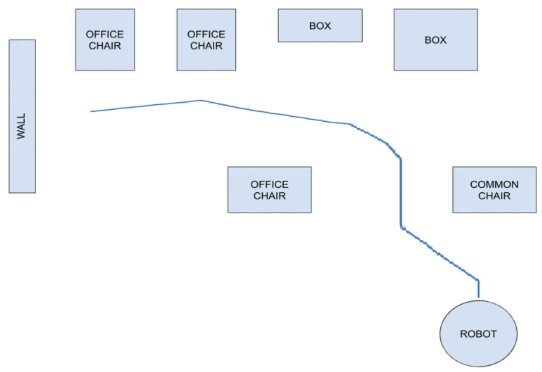
\includegraphics[width=14cm]{pages/OpisRozwiazania/img/wynikPracyArtYOLO.png}
	\caption{Ścieżka i otoczenie, w którym poruszał się robot\cite{yoloAndMobileRobot}}
	\label{rys:sciezkaRobota}
\end{figure}

Na rysunku \ref{rys:sciezkaRobota} widoczne są oznaczone przeszkody, robot oraz przebyta ścieżka. Jak widać w tym i kolejnych prezentowanych przez autorów testach, robot osiągnął docelową pozycje, mimo że nie wiedział o otaczających go przeszkodach. W zaprezentowanym rozwiązaniu, sieć neuronowa musi rozpoznać każdy otaczający robota obiekt, ponieważ w przeciwnym przypadku, ten nie uzna go za przeszkoda i go nie ominie.
W produkcyjnym rozwiązaniu przewidzenie każdego otaczającego robota obiektu jest bardzo trudne.



\subsection{Opis przyjętego rozwiązania}
Jako iż proces samego uczenia sieci neuronowej jak i jej wykorzystanie jest zbyt wymagające dla dowolnego mikrokontrolera przetwarzającego dane to algorytm wykrywający obiekty,
zostanie uruchomiony na laptopie wyposażonym w dedykowaną kartę graficzną RTX3050Ti oraz 6 rdzeniowy procesor AMD Ryzen 5 5600H. 

\begin{figure}[H]
	\centering
	\includegraphics[width=14cm]{pages/OpisRozwiazania/img/SchematOgolny.png}
	\caption{Schemat ogólny przyjętego rozwiązania}
	\label{sch:schematOgolny}
\end{figure}
Jak widać na schemacie z rysunku \ref{sch:schematOgolny}, możemy wydzielić trzy niezależne współpracujące ze sobą elementy.

\textbf{Sterownik} \newline
Zadaniem sterownika jest pobranie, odpowiednie przygotowanie obrazu (np. przeskalowanie go) i przekazanie go do algorytmu wykorzystującego głęboką sieć neuronową. 
Algorytm zwraca pozycję i etykiety wszystkich rozpoznanych na obrazie obiektów, a pozostała część programu wybiera śledzoną etykietę, wyznacza jego pozycję w przestrzeni
roboczej robota i na końcu wysyła odpowiednią komendę.


\textbf{Robot} \newline
Robot zbudowany został w oparciu o laser CNC małej mocy. Maszyna posiada dwie ruchome osie XY z karetką i przyczepionym modułem lasera. Laser i silniki krokowe sterowane są
przy pomocy sterownika opartego na płytce Arduino i odbierającym dane przy pomocy portu USB. Zamiast lasera przy pomocy wydrukowanego na drukarce 3D uchwytu została
zamocowana kamera nagrywająca przestrzeń roboczą, na której stoi urządzenie. Budowa robota została szerzej opisana w kolejnym rozdziale.


\textbf{Kamera} \newline
Jako kamera został wykorzystany telefon komórkowy z systemem Android nagrywający video w rozdzielczości 1920x1080 i 30 klatek na sekundę. W systemie została
zainstalowana aplikacja pozwalająca na strumieniowanie video przy pomocy sieci wifi co ze względu na ciągły ruch kamery znacznie uprościło jej połączenie.
W systemie Windows, na którym uruchomiona jest sieć neuronowa, telefon widoczny jest jako zwykła kamera systemowa.